% \documentclass[handout]{beamer} %"handout" serveix per a treure els \pause
\documentclass{beamer} %"handout" serveix per a treure els \pause
\usepackage{preamble}
\usepackage{../preamble_bib}

\addbibresource{references.bib} % add bibliography file.

\usetheme{Copenhagen}
\usecolortheme{seahorse}


%gets rid of bottom navigation bars
\setbeamertemplate{footline}[frame number]{}

%gets rid of bottom navigation symbols
\setbeamertemplate{navigation symbols}{}

% remove section and subsection from header
\setbeamertemplate{headline}{}

% set right and left margins
\setbeamersize{text margin left=10pt,text margin right=10pt}

\title{2D Turbulence spreading}
\author{
	Víctor Ballester\texorpdfstring{\vspace{0.45cm}\\}{}{\small Supervisors: Alexandros Alexakis (ENS)\texorpdfstring{\\}{}
\hspace{1.5cm} Emmanuel Dormy (ENS)}}
% \institute{Departament de Matemàtiques\\Facultat de Ciències}
\date{July 8, 2024}

% \def\myemph[#1]{
% \begingroup
% \textcolor{\mycolorhighlight}{#1}
% \endgroup}

\begin{document}
\thispagestyle{empty}
\frame[noframenumbering]{\titlepage}
% set the counter to 0
\setcounter{framenumber}{0}
\begin{frame}{Introduction}
	\textbf{Aim:} Understand how turbulence spreads in a 2D incompressible fluid when we constantly inject vortices in the domain.

	The natural questions that arise are:
	\begin{itemize}
		\item Do the vortices injected spread until reaching the boundaries?
		\item If so, which profile does the energy and enstrophy distributions follow?
	\end{itemize}

	\begin{minipage}{0.39\textwidth}
		Additionally, we worked on a \textcolor{\mycolorhighlight}{point vortex model} to compare and observe similarities between the two models.
	\end{minipage}\hspace{0.04\textwidth}
	\begin{minipage}{0.49\textwidth}
		\centering
		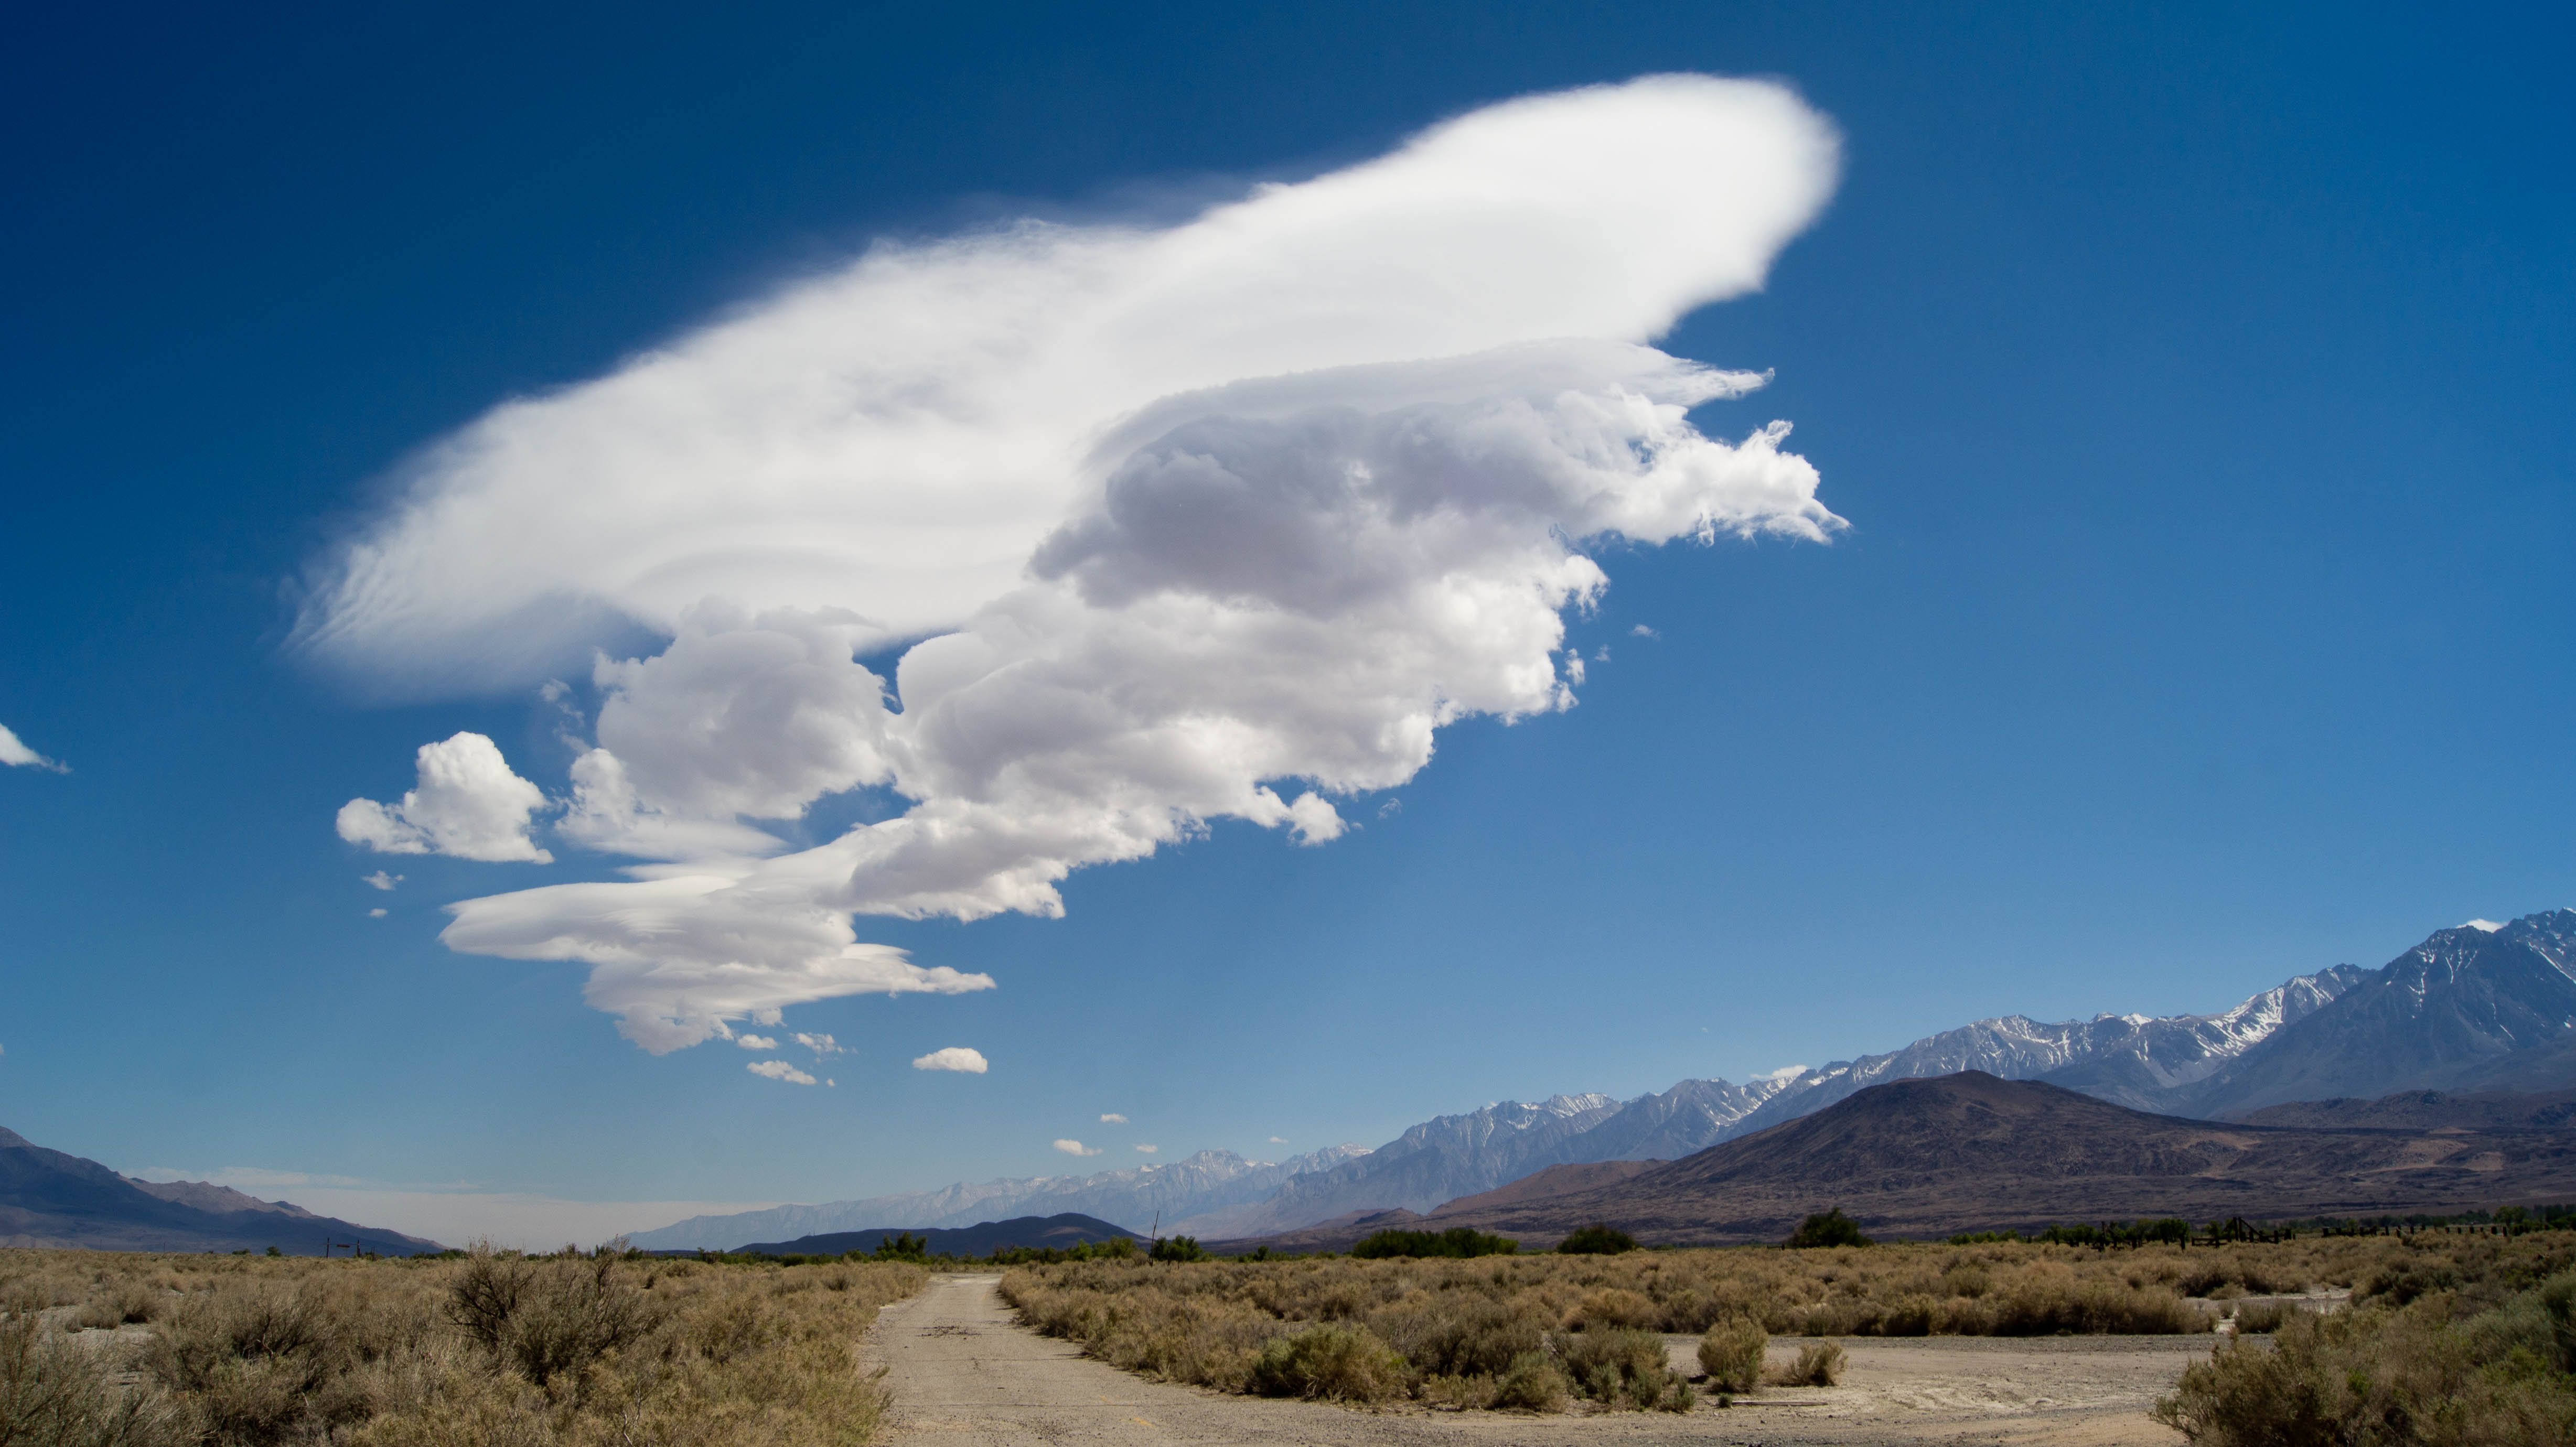
\includegraphics[width=\textwidth]{../images/athmosphere.jpg}
		\captionof{figure}{Turbulence in the atmosphere}
	\end{minipage}
\end{frame}
\begin{frame}{Problem setup (Navier-Stokes)}
	We consider the \textcolor{\mycolorhighlight}{2D incompressible Navier-Stokes equations} which, after nondimensionalizing, read:
	\begin{align*}
		\partial_t \vf{u} + (\vf{u} \cdot \grad) \vf{u} & = -\grad p + \frac{1}{\text{Re}} \Delta \vf{u} + \vf{f} \\
		\divp \vf{u}                                    & = 0
	\end{align*}
	\vspace{-0.8cm}

	\begin{minipage}{0.44\textwidth}
		The force is localized in the center of the domain.

		\begin{itemize}
			\item It injects vortices of size $\sim 1/k_\ell$.
			\item The injection region is a disk of size $\pi/k_r$.
		\end{itemize}
	\end{minipage}\hspace{0.04\textwidth}
	\begin{minipage}{0.44\textwidth}
		\centering
		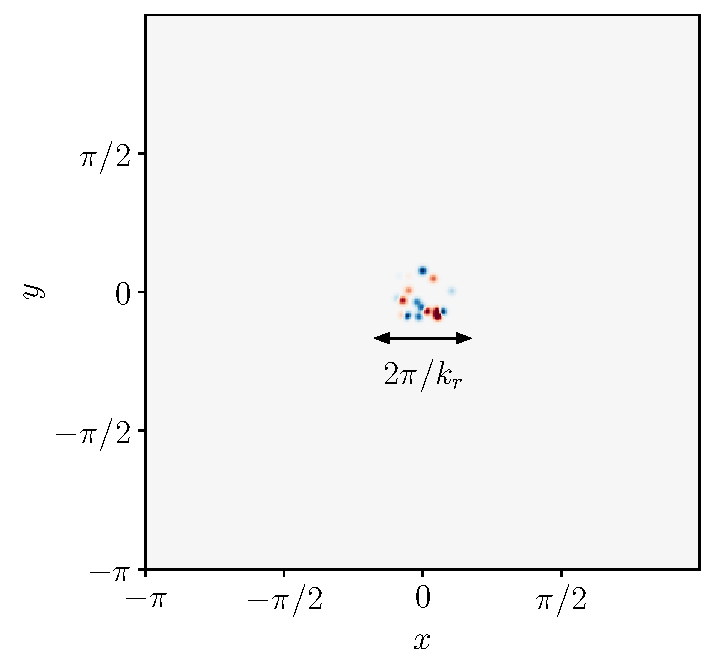
\includegraphics[width=\textwidth]{../images/FlowD_fw.001_arrow.pdf}
		\captionof{figure}{Forcing region for $k_r = 8$}
	\end{minipage}
\end{frame}
\begin{frame}
	Thus, there are three parameters that control the dynamics of the system: $k_\ell$, $k_r$ and $\Re$.

	\textbf{Goal:} Understand the behavior of the system in the limit $\Re\to\infty$ and infinite domain ($k_r\to\infty$).

	We carried out two types of simulations:
	\begin{itemize}
		\item Fully parallel simulations: The domain is split among the processors.
		\item Embarrassingly parallel simulations: Several simulations are run simultaneously, each one in a different processor, in order to produce statistics.
	\end{itemize}
\end{frame}
\begin{frame}
	The following table summarizes the values used in the simulations:

	\begin{table}[ht]
		\centering
		\def\tickgreen{\textcolor{color_green3}{\ding{51}}}
		\def\tickblue{\textcolor{color_blue3}{\ding{51}}}
		% set space between columns
		\setlength{\tabcolsep}{3pt}
		% set space between rows
		\renewcommand{\arraystretch}{1.5}
		{\fontsize{8pt}{10pt}
			\begin{tabular}{c|cccccccccc}
				\diagbox[width=\dimexpr \textwidth/16+2\tabcolsep\relax, height=1cm]{$k_r$}{$\Re$} & 0.25               & 0.5                & 1                  & 2                           & 4                            & 8                            & 16                           & 32                           & 64                  & 128                 \\\hline
				8                                                                                  & \tickgreen$_{512}$ & \tickgreen$_{512}$ & \tickgreen$_{512}$ & \tickgreen\tickblue$_{512}$ & \tickgreen\tickblue$_{1024}$ & \tickgreen\tickblue$_{1024}$ & \tickgreen\tickblue$_{1024}$ & \tickgreen\tickblue$_{2048}$ & \tickgreen$_{2048}$ & \tickgreen$_{4096}$ \\
				16                                                                                 &                    &                    &                    & \tickblue$_{1024}$          & \tickblue$_{2048}$           & \tickgreen\tickblue$_{2048}$ & \tickgreen\tickblue$_{2048}$ & \tickgreen\tickblue$_{2048}$ & \tickgreen$_{4096}$ & \tickgreen$_{4096}$ \\
				32                                                                                 &                    &                    &                    & \tickblue$_{2048}$          & \tickblue$_{4096}$           & \tickgreen\tickblue$_{4096}$ & \tickgreen\tickblue$_{4096}$ & \tickgreen\tickblue$_{4096}$ & \tickgreen$_{8192}$ & \tickgreen$_{8192}$ \\
				64                                                                                 &                    &                    &                    &                             &                              & \tickgreen$_{8192}$          & \tickgreen$_{8192}$          & \tickgreen$_{8192}$          &                     &                     \\
			\end{tabular}}
		\caption{Simulations carried out during the study. \tickgreen = fully parallel simulations,\ \  \tickblue = embarrassingly parallel simulations.}\label{tab:simulations}
	\end{table}

	In all the simulations we set $k_\ell = 4 k_r$.
\end{frame}
\begin{frame}

	\begin{minipage}{0.44\textwidth}
		The quantities monitored during the simulations are the following:
		\begin{align*}
			E_r      & = \sum_{r-\Delta r<\norm{\vf{x}}\leq r} \norm{{\vf{u}}(\vf{x})}^2  \\
			\Omega_r & = \sum_{r-\Delta r<\norm{\vf{x}}\leq r} \abs{{{\omega}}(\vf{x})}^2
		\end{align*}
		which account for the energy and enstrophy in annuli of radius $r$ and width $\Delta r$.
	\end{minipage}\hspace{0.04\textwidth}
	\begin{minipage}{0.44\textwidth}
		\centering
		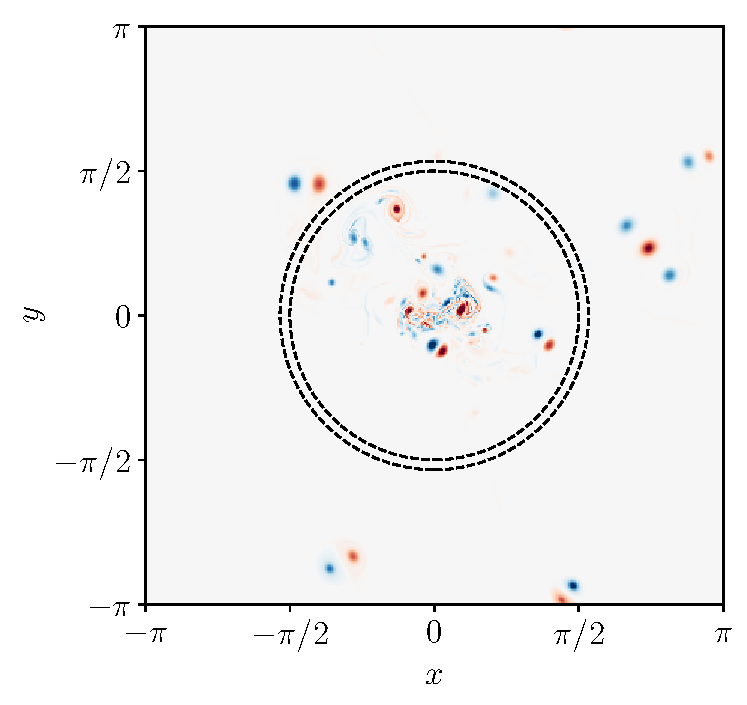
\includegraphics[width=\textwidth]{../images/FlowD_ww.035_annulus.pdf}
	\end{minipage}

	We also defined quantities that measures where most of the energy or enstrophy is located:
	$$
		\mathcal{R}_E^2      = \frac{\sum_{\Delta r<r\leq \pi} r^2 E_r}{\sum_{\Delta r<r\leq \pi} E_r}\qquad 	\mathcal{R}_\Omega^2 = \frac{\sum_{\Delta r<r\leq \pi} r^2 \Omega_r}{\sum_{\Delta r<r\leq \pi} \Omega_r}
	$$
	We call them \emph{mean energy radius} and \emph{mean enstrophy radius}, respectively.
\end{frame}
\begin{frame}{Problem setup (Point vortex)}
	We consider the simplest model of point vortices in 2D, which is based on the evolution by advection of a set of points where the vorticity $\omega$ is singular. At all other points in $\RR^2$, the vorticity is zero.

	At all instants of time $\omega$ can be thought as a sum of Dirac deltas:
	\begin{equation*}
		\omega(\vf{x},t) = \sum_{i=1}^{N} \Gamma_i \delta(\vf{x} - \vf{x}_i(t))
	\end{equation*}
	where $\Gamma_i$ is the circulation of the $i$-th vortex, and $\vf{x}_i(t)$ is its position.

	A set of ODEs can be derived for $\vf{x}_i(t)$ by imposing that they satisfy the 2D incompressible Euler equations:
	\begin{align*}
		\partial_t{\omega} + \vf{u} \cdot \grad {\omega} & = 0 \\
		\divp \vf{u}                                     & = 0
	\end{align*}
\end{frame}
\begin{frame}
	In the point vortex simulations, we input vortices in the center and remove them when they reach the boundaries.

	For this model, we monitor the number of vortices $N_r$ in annuli of radius $r$ and width $\Delta r$, in order to later on give an evolution of the density of number of vortices in rings of radius $r$:
	$$
		\rho_r = \lim_{\Delta r\to 0} \frac{N_r}{2\pi r \Delta r}
	$$

	We also monitor an equivalent \emph{mean radius} $\mathcal{R}_N$ weighted with the number of vortices in each annulus:
	$$
		\mathcal{R}_N^2 = \frac{\sum_{\Delta r<r\leq \pi} r^2 N_r}{\sum_{\Delta r<r\leq \pi} N_r}
	$$
\end{frame}
\begin{frame}{Results}
	\begin{figure}[ht]
		\centering
		\begin{minipage}[t]{0.44\textwidth}
			\centering
			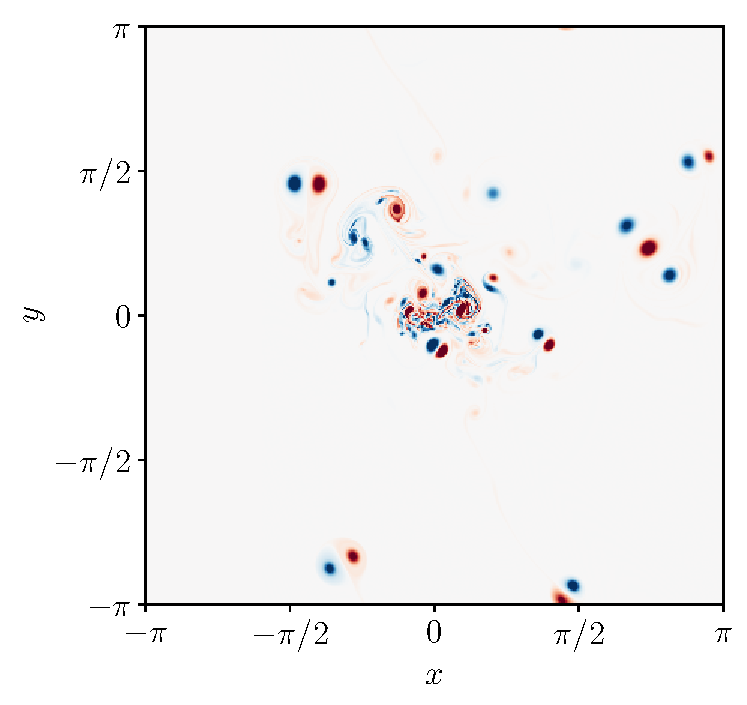
\includegraphics[width=\textwidth]{../images/domainRe128kdn16.pdf}
			\caption{Navier-Stokes simulation with $k_r = 16$ and $\Re = 128$.}
		\end{minipage}\hspace{0.04\textwidth}
		\begin{minipage}[t]{0.44\textwidth}
			\centering
			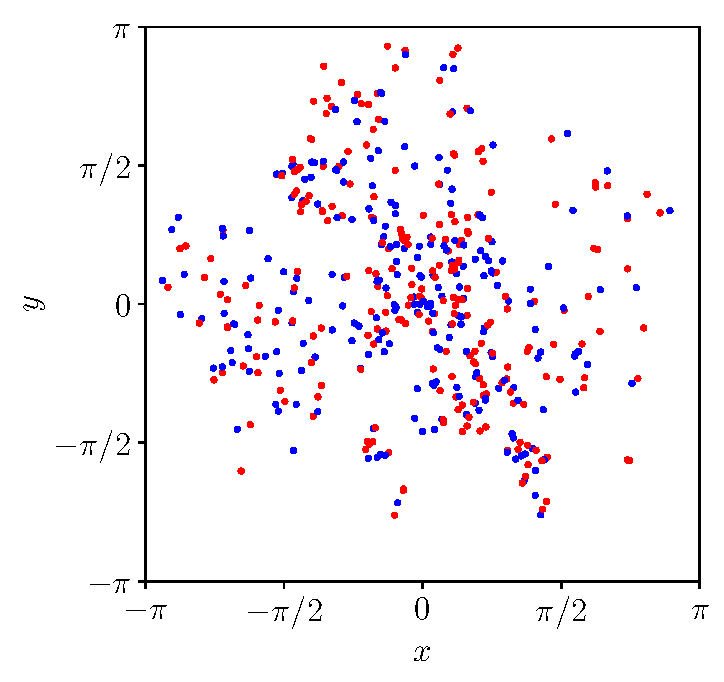
\includegraphics[width=\textwidth]{../images/pointvortices.R4.00440.pdf}
			\caption{Point vortex simulation with $k_r = 16$.}
		\end{minipage}
	\end{figure}
\end{frame}
\begin{frame}{Results (Navier-Stokes)}
	\begin{figure}[ht]
		\centering
		\begin{subfigure}{0.44\textwidth}
			\centering
			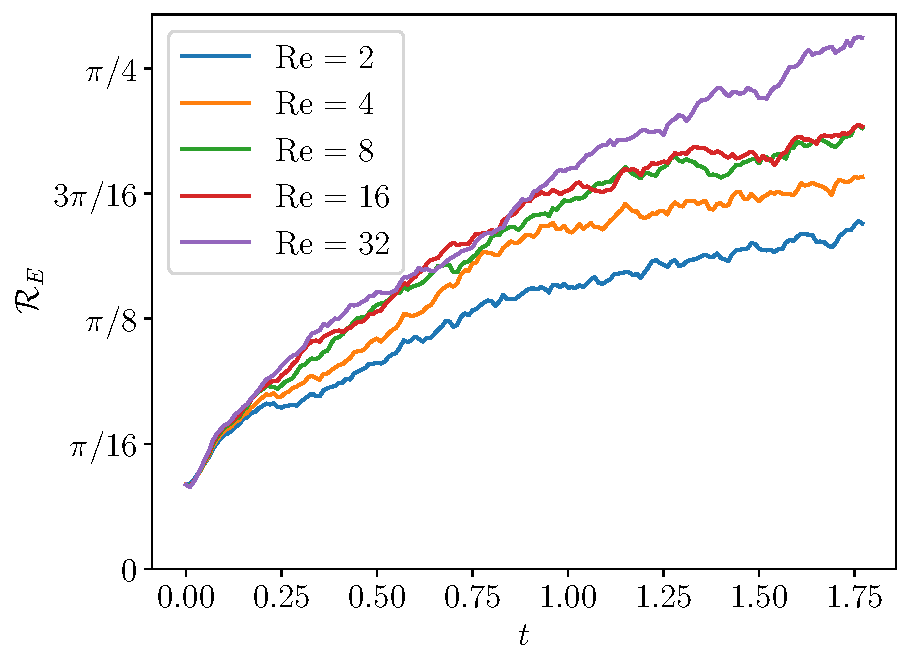
\includegraphics[width=\textwidth]{../images/EnergyMeanRadius_Re.kdn16.pdf}
			\caption{Energy mean radius}
		\end{subfigure}\hspace{0.04\textwidth}
		\begin{subfigure}{0.44\textwidth}
			\centering
			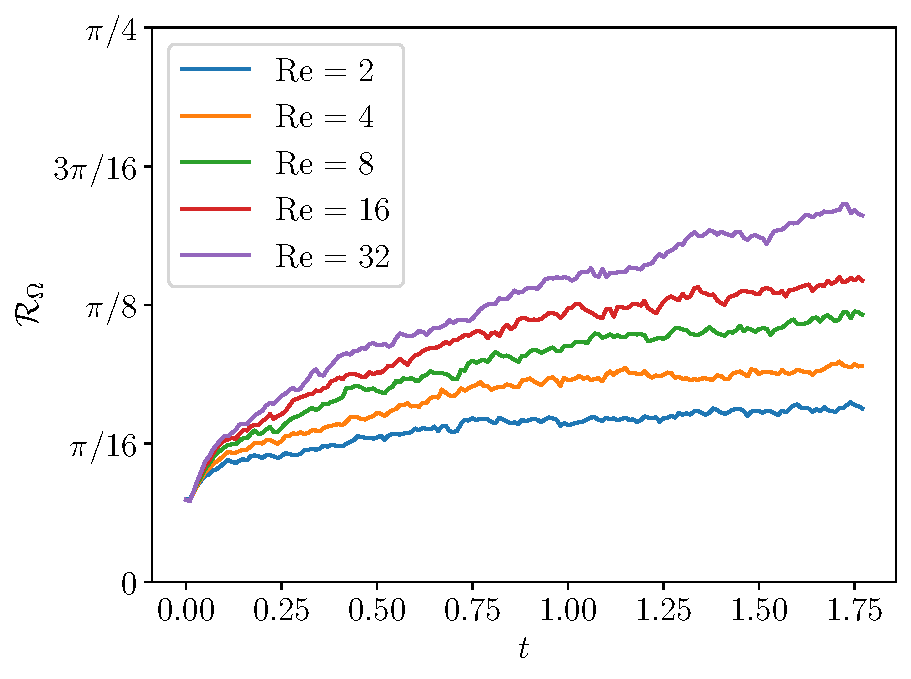
\includegraphics[width=\textwidth]{../images/EnstrophyMeanRadius_Re.kdn16.pdf}
			\caption{Enstrophy mean radius}
		\end{subfigure}
		\caption{Mean energy radius and mean enstrophy radius for several runs varying $\Re$ at $k_r=16$.}
	\end{figure}
	\begin{itemize}
		\item $\mathcal{R}_E$ and $\mathcal{R}_\Omega$ increase with time, which means that vortices spread far from the perturbation region.
		\item The higher the Reynolds number, the faster the spreading.
	\end{itemize}
\end{frame}
\begin{frame}
	\begin{figure}[!ht]
		\centering
		\begin{subfigure}{0.44\textwidth}
			\centering
			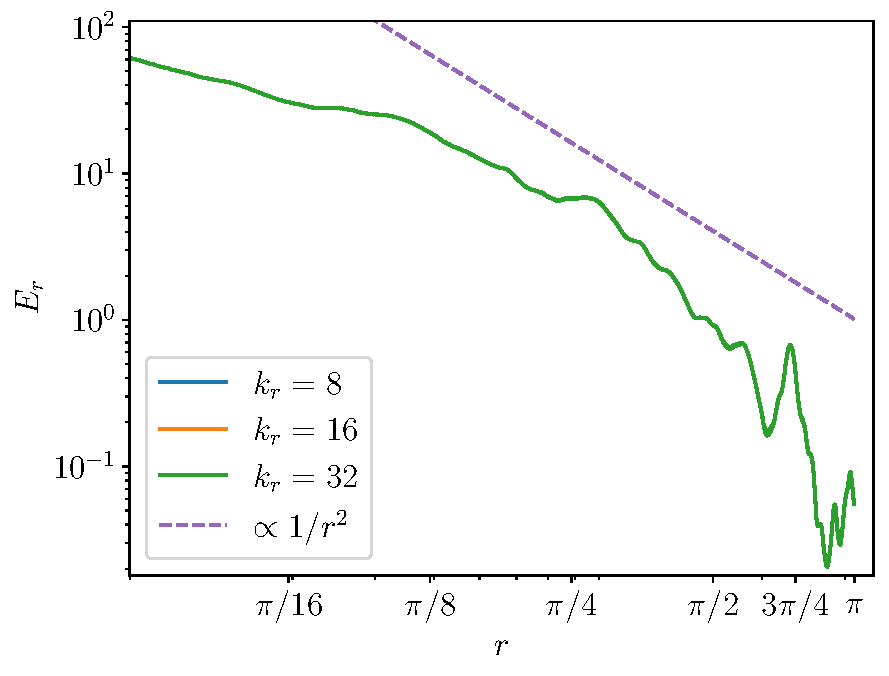
\includegraphics[width=\textwidth]{../images/Energy_kdn.test7.059.pdf}
			\caption{Energy profile}
		\end{subfigure}\hspace{0.04\textwidth}
		\begin{subfigure}{0.44\textwidth}
			\centering
			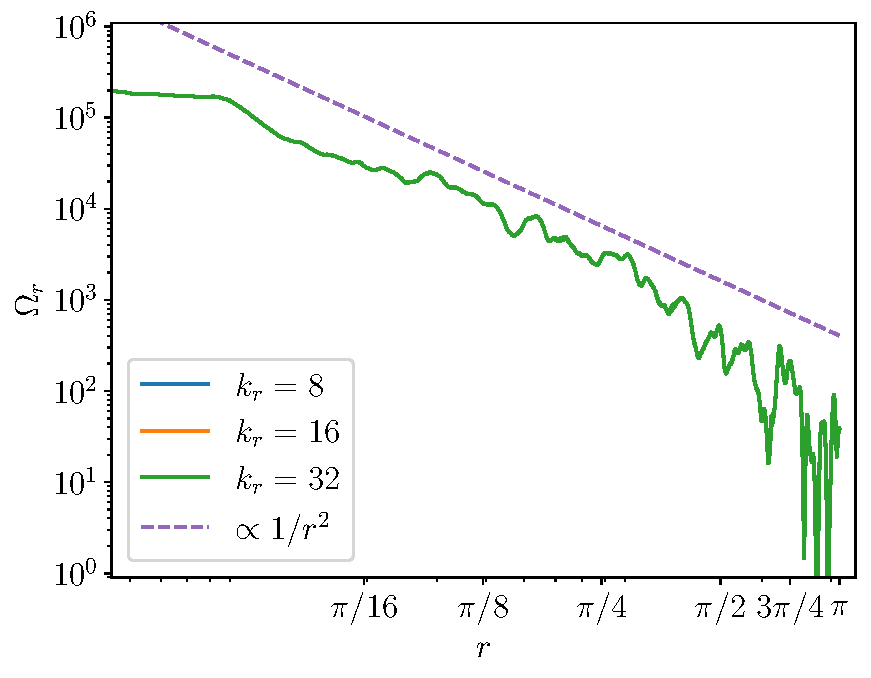
\includegraphics[width=\textwidth]{../images/Enstrophy_kdn.test7.059.pdf}
			\caption{Enstrophy profile}
		\end{subfigure}
		\caption{Energy and enstrophy profiles varying $k_r$ at $t=1.66$ and $\Re=32$.}
	\end{figure}
	\begin{itemize}
		\item Energy plots are smoother, while enstrophy plots are more spiky.
		\item As $k_r$ increases, the apparent power law $A/r^2$ for the enstrophy extends.
	\end{itemize}
\end{frame}
\begin{frame}
	\begin{figure}[!ht]
		\begin{subfigure}{0.44\textwidth}
			\centering
			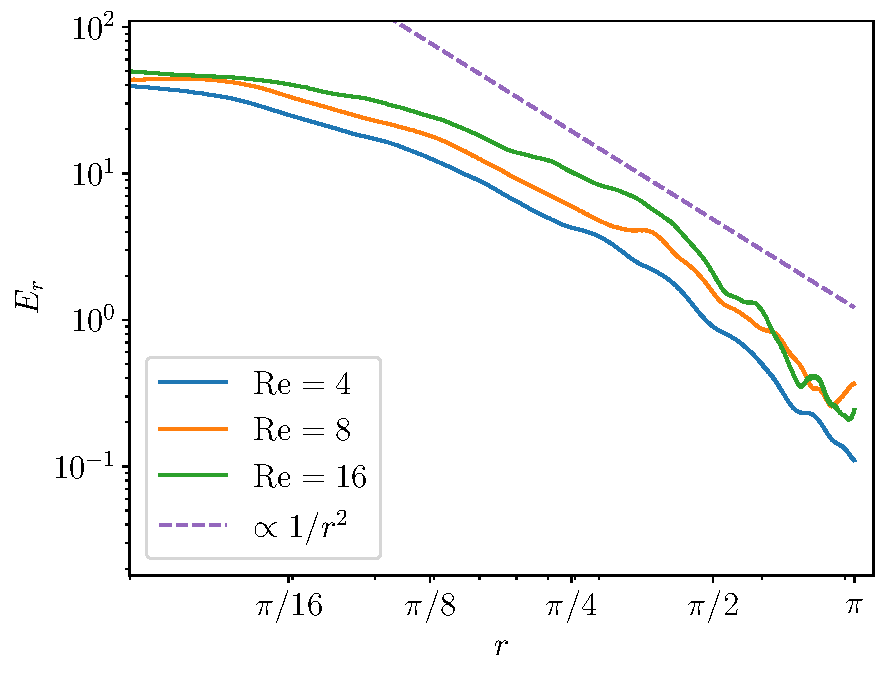
\includegraphics[width=\textwidth]{../images/Energy_Re.kdn16.175.pdf}
			\caption{Energy profile}
		\end{subfigure}\hspace{0.04\textwidth}
		\begin{subfigure}{0.44\textwidth}
			\centering
			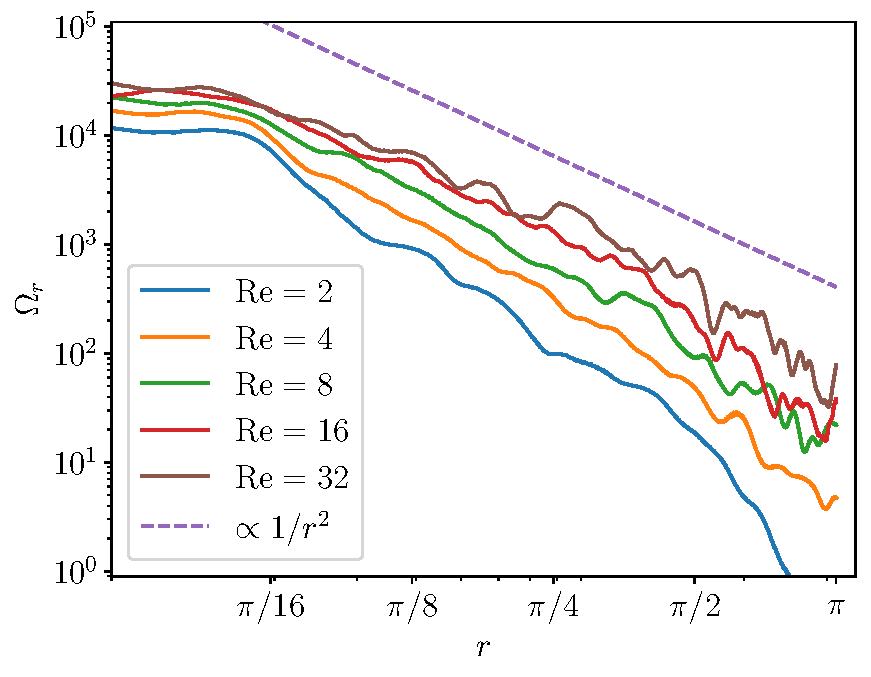
\includegraphics[width=\textwidth]{../images/Enstrophy_Re.kdn16.175.pdf}
			\caption{Enstrophy profile}
		\end{subfigure}
		\caption{Energy and enstrophy profiles varying $\Re$ at $t=1.75$ and $k_r=16$.}
	\end{figure}
	\begin{itemize}
		\item Again, energy plots are smoother than enstrophy plots.
		\item As $\Re$ increases, the magnitudes of both quantities increase due to less dissipation acting on the system.
	\end{itemize}
\end{frame}
\begin{frame}{Results (Point vortex)}
	\begin{figure}[ht]
		\centering
		\begin{minipage}[t]{0.44\textwidth}
			\centering
			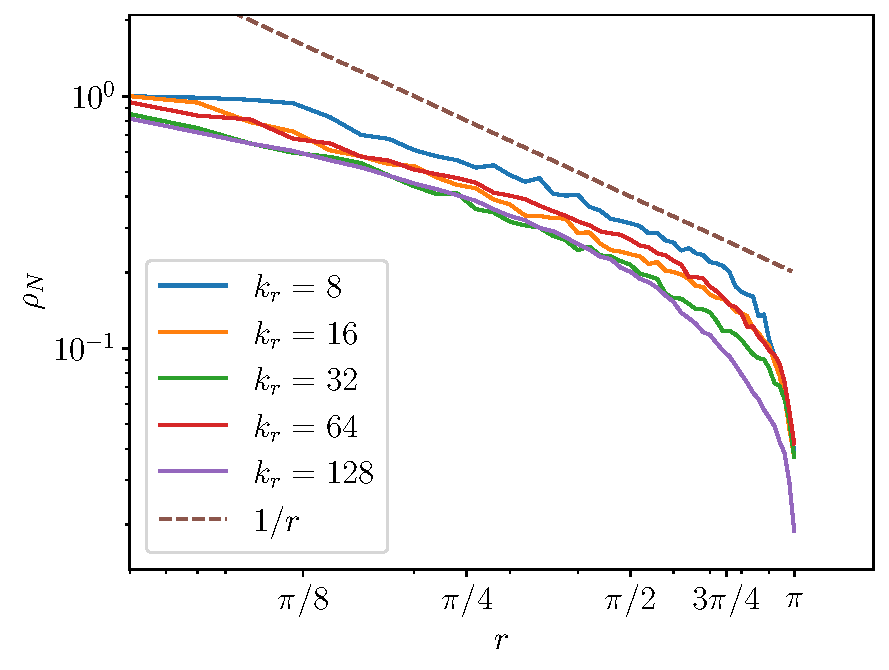
\includegraphics[width=\textwidth]{../images/NumVortices.pdf}
			\caption{Density of the number of vortices as a function of the radius.}
		\end{minipage}\hspace{0.04\textwidth}
		\begin{minipage}[t]{0.44\textwidth}
			\centering
			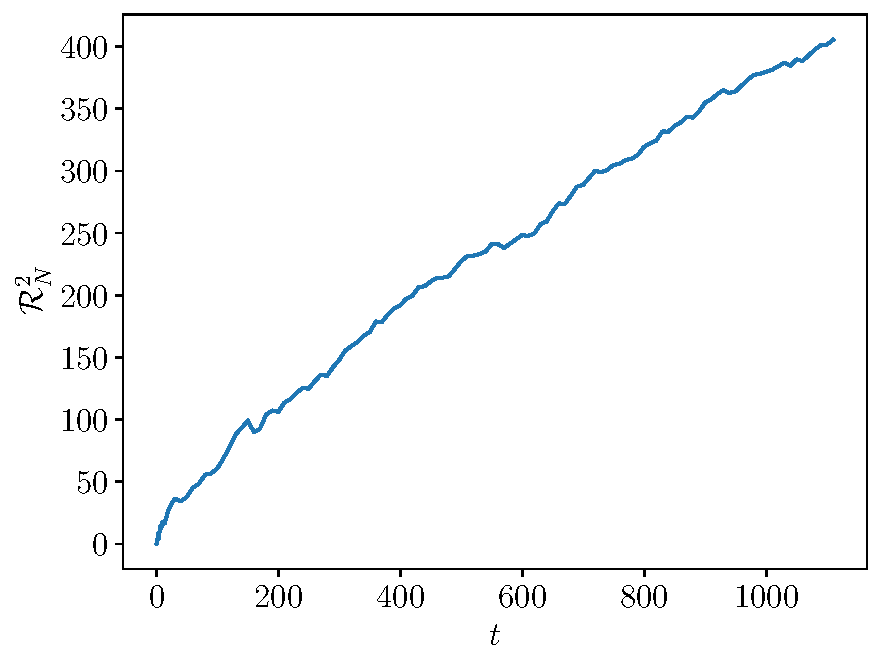
\includegraphics[width=\textwidth]{../images/NumVorticesMeanRadius.pdf}
			\caption{Mean radius weighted with the number of vortices.}		\end{minipage}
	\end{figure}
	\vspace{-0.2cm}
	\begin{itemize}
		\item The density of vortices $\rho_r$ following a power law $A/r$ in the middle range of $r$ implies that the flux of vortices on that region is almost constant.
		\item We observe a monotonous increase of $\mathcal{R}_N$ with time, which resembles the Navier-Stokes case.
	\end{itemize}
\end{frame}
\begin{frame}{Conclusions}
	\begin{itemize}
		\item Energy injected in the center seems to spread across the domain, unlike the 3D case.
		\item The enstrophy seems to follow a power law $A/r^2$, that for large $k_r$, extends to the whole domain.
		\item When a stationary state is reached for the point vortex model, we observe a constant flux of vortices in the middle range of $r$.
	\end{itemize}

	Future improvements:
	\begin{itemize}
		\item Extend the integration time of the Navier-Stokes simulations.
		\item Simulate cases for $k_r= 64$ and higher Reynolds numbers.
		\item Replicate results adding a drag term $-\alpha \vf{u}$ to the equations. Can we conclude the same?
	\end{itemize}
\end{frame}

% \thispagestyle{empty}
% \begin{frame}[noframenumbering]{Bibliography}
% 	\printbibliography
% 	\vspace{4cm}
% \end{frame}
\end{document}
